%********** Chapter 1 **********
\chapter{Introduction}
\section{Overview}

The problem of using cameras to build 3D models of real life environments is
an extremely interesting problem that has been under investigation for many years, the reason for that is that many applications can be built in several
fields using such a technology, also advances in both cameras and hardware equipments encourage researchers and developers to take the problem to new levels building models more accurately and faster

In our project, we use the commerically well-known and available Kinect to build Simultaneous Localization and Mapping system known as SLAM, this system allows
a user to build 3D models of an indoor environment using a hand-held Kinect.

\section{History}

2D images obtained from ordinary cameras have been widely used to build 3D models of real life objects using the well known pipeline of Structure from Motion (SFM), but challenges exist in constructing models with accurate real distances maintained.

Anyway the introduction of laser scanners has provided more accurate information about the nature of scenes and objects especially surfaces with complex structure, the complexity of laser scanners and their high cost that can be up to tens of thousands of dollars make them only suitable for professionals.

Between the ordinary 2D camers and the expensive laser scanners, new cheap cameras (costs only hundreds of dollars) named RGB-D cameras have emerged in the market starting from 2009 such as the Kinect camera that was named initialy Project Natal, and although the Kinect was targeting the gaming industry, a wave of hacks exploiting the capabilities of Kinect in different fields such as 3D reconstruction has proved that despite the low sepecifications of the device it still can be used to produce results are useful for many users.

\begin{figure}[ht]
\begin{minipage}[b]{0.5\linewidth}
\centering
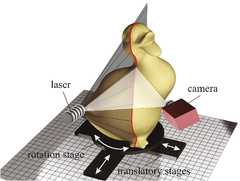
\includegraphics[scale=2.5,keepaspectratio=true]{chap1/intro.png}
\caption{Using Laser Scanners}
\label{fig:intro}
\end{minipage}
\hspace{0.5cm}
\begin{minipage}[b]{0.5\linewidth}
\centering
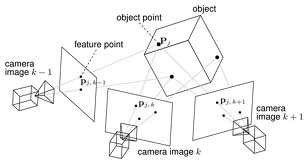
\includegraphics[scale=0.5,keepaspectratio=true]{chap1/SFM.jpg}
\caption{Structure From Motion}
\label{fig:SFM}
\end{minipage}
\end{figure}

\section{Organization of this Book}

This book is divided into the following 11 chapters:

\hbox{}
Chapter 1: Introduction - introduces the problem we are trying to solve and 
brief glimpse of related work

\hbox{}
Chapter 2: Background - provides a formal definition of SLAM problem and gives an overview on the suggested pipeline explained in detail in later chapters

\hbox{}
Chapter 3: System Analysis and Design - explains the top level analysis of the system and how components integrate using UML diagrams

\hbox{}
Chapter 4: Using Kinect - explains our choice of Kinect as the scanning camera and details its sepecifications and history

\hbox{}
Chapter 5: Feature Extraction and Matching - compares two different methods that we used to track features from consecutive frames

\hbox{}
Chapter 6: Camera Tranformation Calculation - explains the methods used to calculate a transformation between the correspondences obtained from feature matching

\hbox{}
Chapter 7: Loop Closure and Global Optimization - explains how we solved the problem of scene revisiting and accumlative error handling

\hbox{}
Chapter 8: Refinement and Surface construction - discusses the different techniques that are used in enhancing the build 3D model

\hbox{}
Chapter 9: Segmentation - demonstrates applying segmentation can be used to perform editing on the built 3D models

\hbox{}
Chapter 10: User Interface - describes the User Interface that a user uses to perform the different tasks the system provides

\hbox{}
Chapter 11: Conclusions and Future Work - explains our conclusions and how this project can develop further in the future

%********** End of chapter **********
